\documentclass{anstrans}
%%%%%%%%%%%%%%%%%%%%%%%%%%%%%%%%%%%
\title{The impact of xenon-135 poisoning on Load Following Transatomic Power 
Molten Salt Reactor}

\author{Andrei Rykhlevskii, Daniel O'grady, Tomasz Kozlowski, Kathryn Huff}

\institute{
        Department of Nuclear, Plasma, and Radiological Engineering, University 
        of Illinois at Urbana-Champaign \break
        Urbana, IL
}

\email{andreir2@illinois.edu}

%%%% packages and definitions (optional)
\usepackage{graphicx} % allows inclusion of graphics
\usepackage{caption}  % allows center figures caption
\usepackage{booktabs} % nice rules (thick lines) for tables
\usepackage{microtype} % improves typography for PDF
\usepackage[section]{placeins}

\usepackage[acronym,toc]{glossaries}  % acronyms inclusion
%\newacronym{<++>}{<++>}{<++>}
\newacronym[longplural={metric tons of heavy metal}]{MTHM}{MTHM}{metric ton of heavy metal}
\newacronym{ABM}{ABM}{agent-based modeling}
\newacronym{ACDIS}{ACDIS}{Program in Arms Control \& Domestic and International Security}
\newacronym{AHTR}{AHTR}{Advanced High Temperature Reactor}
\newacronym{ANDRA}{ANDRA}{Agence Nationale pour la gestion des D\'echets RAdioactifs, the French National Agency for Radioactive Waste Management}
\newacronym{ANL}{ANL}{Argonne National Laboratory}
\newacronym{ANS}{ANS}{American Nuclear Society}
\newacronym{API}{API}{application programming interface}
\newacronym{ARE}{ARE}{Aircraft Reactor Experiment}
\newacronym{ARFC}{ARFC}{Advanced Reactors and Fuel Cycles}
\newacronym{ASME}{ASME}{American Society of Mechanical Engineers}
\newacronym{ATWS}{ATWS}{Anticipated Transient Without Scram}
\newacronym{BOL}{BOL}{Beginning of Life}
\newacronym{BDBE}{BDBE}{Beyond Design Basis Event}
\newacronym{BIDS}{BIDS}{Berkeley Institute for Data Science}
\newacronym{BWR}{BWR}{Boiling Water Reactor}
\newacronym{CAFCA}{CAFCA}{ Code for Advanced Fuel Cycles Assessment }
\newacronym{CDTN}{CDTN}{Centro de Desenvolvimento da Tecnologia Nuclear}
\newacronym{CFD}{CFD}{Computational Fluid Dynamics}
\newacronym{CEA}{CEA}{Commissariat \`a l'\'Energie Atomique et aux \'Energies Alternatives}
\newacronym{CI}{CI}{continuous integration}
\newacronym{CNEN}{CNEN}{Comiss\~{a}o Nacional de Energia Nuclear}
\newacronym{CNERG}{CNERG}{Computational Nuclear Engineering Research Group}
\newacronym{COSI}{COSI}{Commelini-Sicard}
\newacronym{COTS}{COTS}{commercial, off-the-shelf}
\newacronym{CSNF}{CSNF}{commercial spent nuclear fuel}
\newacronym{CTAH}{CTAHs}{Coiled Tube Air Heaters}
\newacronym{CUBIT}{CUBIT}{CUBIT Geometry and Mesh Generation Toolkit}
\newacronym{CURIE}{CURIE}{Centralized Used Fuel Resource for Information Exchange}
\newacronym{CR}{CR}{conversion ratio}
\newacronym{DAG}{DAG}{directed acyclic graph}
\newacronym{DANESS}{DANESS}{Dynamic Analysis of Nuclear Energy System Strategies}
\newacronym{DBE}{DBE}{Design Basis Event}
\newacronym{DESAE}{DESAE}{Dynamic Analysis of Nuclear Energy Systems Strategies}
\newacronym{DHS}{DHS}{Department of Homeland Security}
\newacronym{DOE}{DOE}{Department of Energy}
\newacronym{DRACS}{DRACS}{Direct Reactor Auxiliary Cooling System}
\newacronym{DRE}{DRE}{dynamic resource exchange}
\newacronym{DSNF}{DSNF}{DOE spent nuclear fuel}
\newacronym{DYMOND}{DYMOND}{Dynamic Model of Nuclear Development }
\newacronym{EBS}{EBS}{Engineered Barrier System}
\newacronym{EDF}{EDF}{Électricité de France}
\newacronym{EDZ}{EDZ}{Excavation Disturbed Zone}
\newacronym{EOL}{EOL}{End of Life}
\newacronym{EIA}{EIA}{U.S. Energy Information Administration}
\newacronym{EPA}{EPA}{Environmental Protection Agency}
\newacronym{EPR}{EPR}{European Pressurized Reactors}
\newacronym{EP}{EP}{Engineering Physics}
\newacronym{EU}{EU}{European Union}
\newacronym{FCO}{FCO}{Fuel Cycle Options}
\newacronym{FCT}{FCT}{Fuel Cycle Technology}
\newacronym{FEHM}{FEHM}{Finite Element Heat and Mass Transfer}
\newacronym{FEPs}{FEPs}{Features, Events, and Processes}
\newacronym{FHR}{FHR}{Fluoride-Salt-Cooled High-Temperature Reactor}
\newacronym{FLiBe}{FLiBe}{Fluoride-Lithium-Beryllium}
\newacronym{FP}{FP}{Fission Product}
\newacronym{GDSE}{GDSE}{Generic Disposal System Environment}
\newacronym{GDSM}{GDSM}{Generic Disposal System Model}
\newacronym{GENIUSv1}{GENIUSv1}{Global Evaluation of Nuclear Infrastructure Utilization Scenarios, Version 1}
\newacronym{GENIUSv2}{GENIUSv2}{Global Evaluation of Nuclear Infrastructure Utilization Scenarios, Version 2}
\newacronym{GENIUS}{GENIUS}{Global Evaluation of Nuclear Infrastructure Utilization Scenarios}
\newacronym{GPAM}{GPAM}{Generic Performance Assessment Model}
\newacronym{GRSAC}{GRSAC}{Graphite Reactor Severe Accident Code}
\newacronym{GUI}{GUI}{graphical user interface}
\newacronym{HLW}{HLW}{high level waste}
\newacronym{HPC}{HPC}{high-performance computing}
\newacronym{HTC}{HTC}{high-throughput computing}
\newacronym{HTGR}{HTGR}{High Temperature Gas-Cooled Reactor}
\newacronym{IAEA}{IAEA}{International Atomic Energy Agency}
\newacronym{IEMA}{IEMA}{Illinois Emergency Mangament Agency}
\newacronym{IHLRWM}{IHLRWM}{International High Level Radioactive Waste Management}
\newacronym{INL}{INL}{Idaho National Laboratory}
\newacronym{IPRR1}{IRP-R1}{Instituto de Pesquisas Radioativas Reator 1}
\newacronym{IRP}{IRP}{Integrated Research Project}
\newacronym{ISFSI}{ISFSI}{Independent Spent Fuel Storage Installation}
\newacronym{ISRG}{ISRG}{Independent Student Research Group}
\newacronym{JFNK}{JFNK}{Jacobian-Free Newton Krylov}
\newacronym{LANL}{LANL}{Los Alamos National Laboratory}
\newacronym{LBNL}{LBNL}{Lawrence Berkeley National Laboratory}
\newacronym{LCOE}{LCOE}{levelized cost of electricity}
\newacronym{LEU}{LEU}{low-enriched uranium}
\newacronym{LDRD}{LDRD}{laboratory directed research and development}
\newacronym{LFR}{LFR}{Lead-Cooled Fast Reactor}
\newacronym{LLNL}{LLNL}{Lawrence Livermore National Laboratory}
\newacronym{LMFBR}{LMFBR}{Liquid Metal Fast Breeder Reactor}
\newacronym{LOFC}{LOFC}{Loss of Forced Cooling}
\newacronym{LOHS}{LOHS}{Loss of Heat Sink}
\newacronym{LOLA}{LOLA}{Loss of Large Area}
\newacronym{LP}{LP}{linear program}
\newacronym{LWR}{LWR}{Light Water Reactor}
\newacronym{MAGNOX}{MAGNOX}{Magnesium Alloy Graphie Moderated Gas Cooled Uranium Oxide Reactor}
\newacronym{MA}{MA}{minor actinide}
\newacronym{MCNP}{MCNP}{Monte Carlo N-Particle code}
\newacronym{MILP}{MILP}{mixed-integer linear program}
\newacronym{MIT}{MIT}{the Massachusetts Institute of Technology}
\newacronym{MOAB}{MOAB}{Mesh-Oriented datABase}
\newacronym{MOOSE}{MOOSE}{Multiphysics Object-Oriented Simulation Environment}
\newacronym{MOSART}{MOSART}{Molten Salt Actinide Recycler and Transmuter}
\newacronym{MOX}{MOX}{mixed oxide}
\newacronym{MPI}{MPI}{Message Passing Interface}
\newacronym{MSBR}{MSBR}{Molten Salt Breeder Reactor}
\newacronym{MSFR}{MSFR}{Molten Salt Fast Reactor}
\newacronym{MSRE}{MSRE}{Molten Salt Reactor Experiment}
\newacronym{MSR}{MSR}{Molten Salt Reactor}
\newacronym{NAGRA}{NAGRA}{National Cooperative for the Disposal of Radioactive Waste}
\newacronym{NEAMS}{NEAMS}{Nuclear Engineering Advanced Modeling and Simulation}
\newacronym{NEUP}{NEUP}{Nuclear Energy University Programs}
\newacronym{NFCSim}{NFCSim}{Nuclear Fuel Cycle Simulator}
\newacronym{NGNP}{NGNP}{Next Generation Nuclear Plant}
\newacronym{NMWPC}{NMWPC}{Nuclear MW Per Capita}
\newacronym{NNSA}{NNSA}{National Nuclear Security Administration}
\newacronym{NPP}{NPP}{Nuclear Power Plant}
\newacronym{NPRE}{NPRE}{Department of Nuclear, Plasma, and Radiological Engineering}
\newacronym{NQA1}{NQA-1}{Nuclear Quality Assurance - 1}
\newacronym{NRC}{NRC}{Nuclear Regulatory Commission}
\newacronym{NSF}{NSF}{National Science Foundation}
\newacronym{NSSC}{NSSC}{Nuclear Science and Security Consortium}
\newacronym{NUWASTE}{NUWASTE}{Nuclear Waste Assessment System for Technical Evaluation}
\newacronym{NWF}{NWF}{Nuclear Waste Fund}
\newacronym{NWTRB}{NWTRB}{Nuclear Waste Technical Review Board}
\newacronym{OCRWM}{OCRWM}{Office of Civilian Radioactive Waste Management}
\newacronym{OOP}{OOP}{Object-Orienting Programming}
\newacronym{ORION}{ORION}{ORION}
\newacronym{ORNL}{ORNL}{Oak Ridge National Laboratory}
\newacronym{PARCS}{PARCS}{Purdue Advanced Reactor Core Simulator}
\newacronym{PBAHTR}{PB-AHTR}{Pebble Bed Advanced High Temperature Reactor}
\newacronym{PBFHR}{PB-FHR}{Pebble-Bed Fluoride-Salt-Cooled High-Temperature Reactor}
\newacronym{PEI}{PEI}{Peak Environmental Impact}
\newacronym{PH}{PRONGHORN}{PRONGHORN}
\newacronym{PRIS}{PRIS}{Power Reactor Information System}
\newacronym{PRKE}{PRKE}{Point Reactor Kinetics Equations}
\newacronym{PSPG}{PSPG}{Pressure-Stabilizing/Petrov-Galerkin}
\newacronym{PWAR}{PWAR}{Pratt and Whitney Aircraft Reactor}
\newacronym{PWR}{PWR}{Pressurized Water Reactor}
\newacronym{PyNE}{PyNE}{Python toolkit for Nuclear Engineering}
\newacronym{PyRK}{PyRK}{Python for Reactor Kinetics}
\newacronym{QA}{QA}{quality assurance}
\newacronym{RDD}{RD\&D}{Research Development and Demonstration}
\newacronym{RD}{R\&D}{Research and Development}
\newacronym{REE}{REE}{rare earth element}
\newacronym{RELAP}{RELAP}{Reactor Excursion and Leak Analysis Program}
\newacronym{RIA}{RIA}{Reactivity Insertion Accident}
\newacronym{RIF}{RIF}{Region-Institution-Facility}
\newacronym{SFR}{SFR}{Sodium-Cooled Fast Reactor}
\newacronym{SINDAG}{SINDA{\textbackslash}G}{Systems Improved Numerical Differencing Analyzer $\backslash$ Gaski}
\newacronym{SKB}{SKB}{Svensk K\"{a}rnbr\"{a}nslehantering AB}
\newacronym{SNF}{SNF}{spent nuclear fuel}
\newacronym{SNL}{SNL}{Sandia National Laboratory}
\newacronym{STC}{STC}{specific temperature change}
\newacronym{SUPG}{SUPG}{Streamline-Upwind/Petrov-Galerkin}
\newacronym{SVF}{SVF}{salt volume fraction}
\newacronym{SWF}{SWF}{Separations and Waste Forms}
\newacronym{SWU}{SWU}{Separative Work Unit}
\newacronym{TAP}{TAP}{Transatomic Power}
\newacronym{TRIGA}{TRIGA}{Training Research Isotope General Atomic}
\newacronym{TRISO}{TRISO}{Tristructural Isotropic}
\newacronym{TSM}{TSM}{Total System Model}
\newacronym{TSPA}{TSPA}{Total System Performance Assessment for the Yucca Mountain License Application}
\newacronym{ThOX}{ThOX}{thorium oxide}
\newacronym{UFD}{UFD}{Used Fuel Disposition}
\newacronym{UML}{UML}{Unified Modeling Language}
\newacronym{UOX}{UOX}{uranium oxide}
\newacronym{UQ}{UQ}{uncertainty quantification}
\newacronym{US}{US}{United States}
\newacronym{UW}{UW}{University of Wisconsin}
\newacronym{VISION}{VISION}{the Verifiable Fuel Cycle Simulation Model}
\newacronym{VVER}{VVER}{Voda-Vodyanoi Energetichesky Reaktor (Russian Pressurized Water Reactor)}
\newacronym{VV}{V\&V}{verification and validation}
\newacronym{WIPP}{WIPP}{Waste Isolation Pilot Plant}
\newacronym{YMR}{YMR}{Yucca Mountain Repository Site}


\usepackage{tabularx} % for nice wrapping of table text

\makeglossaries

\graphicspath{{figures/}}

\newcommand{\SN}{S$_N$}
\renewcommand{\vec}[1]{\bm{#1}} %vector is bold italic
\newcommand{\vd}{\bm{\cdot}} % slightly bold vector dot
\newcommand{\grad}{\vec{\nabla}} % gradient
\newcommand{\ud}{\mathop{}\!\mathrm{d}} % upright derivative symbol

\begin{document}
%%%%%%%%%%%%%%%%%%%%%%%%%%%%%%%%%%%%%%%%%%%%%%%%%%%%%%%%%%%%%%%%%%%%%%%%%%%%%%%%
\section{Introduction}
First-of-kind civil \gls{MSR} was developed, built and operated in \gls{ORNL}  
in 1960s. It was called \gls{MSRE} and at the moment is the
only one operated 
\gls{MSR} worldwide. Based on experience from this experiment first commercial
\gls{MSBR} was designed in early 1970s. In the thermal spectrum \gls{MSR}, 
fluorides of fissile and/or fertile materials (i.e.
UF$_4$, PuF$_3$ and/or 
ThF$_4$) are mixed with carrier salts (i.e. LiF) to form a liquid fuel
which 
is circulated in a loop-type primary circuit which lead to following 
advantages over traditional solid-fueled reactors: (1) relatively low pressure 
in the primary loop; (2) strong negative thermal feedback; (3) passive decay 
heat cooling; (4) reduced fuel fabrication costs; (5) online refueling and 
reprocessing \cite{haubenreich_experience_1970}.

Nevertheless, cost-competitiveness of such innovative designs in the current 
domestic energy market may only be feasible with load-following operation. 
Load following operation has the potential to dramatically increase the 
commercial competitiveness of nuclear power. Due to increasing penetration of 
renewables on the electric grid, base-load operation carries the risk of 
correspondingly frequent negative electric energy pricing. Thus, 
responsiveness to net electricity demand is essential to market relevance for
new designs \cite{energy_information_administration_u.s._2016}.

The main physical effect that limit the possibilities of power variations in a 
conventional \gls{LWR} is fission product poisoning, especially the xenon  
effect (few hours after the change in the reactor power level).  The 
$^{135}$Xe is the most powerful known neutron absorber (average cross section 
for thermal neutrons approximately $10^6$ barns) with half-life  
$\tau_{1/2}=9.17h$ and yield for $^{235}$U fission about 6.3\%. The vast 
majority of xenon-135 (6.1\%) is produced from another fission product - 
$^{135}$I ($\tau_{1/2}=6.6h$) \cite{lokhov_technical_2011}. Under normal 
operating conditions, the $^{135}$Xe is burned in the reactor core as it is 
produced, so while it has a negative impact on the neutron economy, balancing 
the reactor controls can compensate for its effect. The difficulty comes when 
the reactor power is reduced and there are fewer neutrons to burn out the 
$^{135}$Xe, so its concentration increases and further suppresses reactor 
power. In this case, the core takes some time to recover from the power 
reduction impact of $^{135}$Xe. This response to changing power levels, 
particularly from higher to lower power levels, dramatically slows the 
reactor’s response to power demands. Potentially, $^{135}$Xe removal during 
reactor operation would allow more flexibly vary power levels to follow power 
demands, typically referred as `load following'.

The \gls{TAP} \gls{MSR} design is a 1250 MW$_{th}$ liquid-fueled reactor has 
been selected as a prototype of modern \gls{MSR}. The \gls{TAP} is an 
intermediate spectrum reactor designed to be started with high-essay \gls{LEU} 
uranium as initial fissile load. This work presents modeling and simulation of 
load following power transient operation of the \gls{TAP} \gls{MSR}. We 
compared these results with well-studied \gls{PWR} behavior. This study 
focuses on the $^{135}$Xe/$^{135}$I balance in the \gls{TAP} core and its 
effect on the reactor performance. Another feature of the \gls{MSR}, its 
circulating liquid fuel and
corresponding delayed neutron precursor drift, is 
not treated
here.

Much of the analysis herein used a full-core 3-D model of the \gls{TAP}  
developed using the continuous-energy Serpent 2 Monte Carlo reactor physics 
software. The \gls{PWR} transient analysis has been done for single-assembly 
model with burnable poison (gadolinium) provided with Serpent 
\cite{leppanen_serpent_2015}. All calculations presented in this paper were 
performed using the Serpent 2 code version 2.1.31 with JEFF-3.1.2 nuclear data 
\cite{oecd/nea_data_bank_jeff-3.1.2_2014}.
%%%%%%%%%%%%%%%%%%%%%%%%%%%%%%%%%%%%%%%%%%%%%%%%%%%%%%%%%%%%%%%%%%%%%%%%%%%%%%%%
\section{Description of the actual work}
\subsection{Transatomic Power reactor design description}
The \gls{TAP} design is very similar to original \gls{MSRE} design developed 
by \gls{ORNL} \cite{haubenreich_experience_1970} but has two major  
innovations: 
the fuel salt composition and the moderator. The \gls{MSRE}'s 
LiF-BeF$_2$-ZrF$_4$-UF$_4$ salt has been substituted with LiF-UF$_4$ salt 
which 
allows for an increase in the uranium concentration within the fuel salt from 
0.9 to 
27.5\% while maintaining a relatively low melting point (490$^{\circ}$C 
compared 
with 434$^{\circ}$C for the original \gls{MSRE}'s salt) 
\cite{betzler_two-dimensional_2016}. The graphite has a very high 
thermal scattering cross section which makes it a perfect moderator but has 
a few major drawbacks: 
(1) the low lethargy gain per collision requires a large volume of moderator 
to be present to reach criticality, which leads to a larger core and obstructs 
the core power density; (2) even special 
reactor-grade graphite has relatively high porosity, consequently, it holds
gaseous \glspl{FP} 
(e.g., tritium, xenon) in pores; (3) the reactor graphite lifespan in a 
commercial 
reactor is about 10 years \cite{robertson_conceptual_1971}. To resolve these 
issues, the \gls{TAP} concept uses another 
moderator, namely, zirconium hydride, allowing for a more compact core and a 
significant increase in power density. These two innovative design choices,  
together with a configurable moderator 
(the moderator-to-fuel ratio can be changed during regular maintenance 
shutdown), 
facilitate the commercial deployment of this conceptual design in the current 
commercially available 5\% \gls{LEU} fuel cycle. 

The \gls{TAP} \gls{MSR} primary loop contains the reactor core volume 
(including 
the zirconium hydride moderator rods with silicone carbide cladding), pumps, 
and 
primary heat exchanger. Pumps circulate the LiF-(Act)F$_4$ 
fuel salt through the primary loop. The pumps, vessels, tanks, and piping are 
made of a nickel-based alloy (similar to Hastelloy-N\footnote{ Hastelloy-N  
is 	very common in reactors now but have been studied and developed at  
\gls{ORNL} in a program that started in 1950s.}), which is highly resistant to 
corrosion in various molten salt environments. Inside the reactor vessel, in 
close proximity to the zirconium hydride moderator rods, the fuel salt is in a 
critical configuration and generates heat. Table~\ref{tab:tap_tab} contains 
details of the \gls{TAP} system design which are taken from technical white 
paper \cite{transatomic_power_corporation_technical_2016} and a neutronics 
overview \cite{transatomic_power_corporation_neutronics_2016} as well as 
\gls{ORNL} analysis of the \gls{TAP} design 
\cite{betzler_two-dimensional_2016, betzler_assessment_2017}. 
%%%%%%%%%%%%%%%%%%%%%%%%%%%%%%%%%%%%%%%%
\begin{table}[h!]
	\caption{Summary of principal data for the \gls{TAP} \gls{MSR} 
		(reproduced from \cite{transatomic_power_corporation_technical_2016, 
		betzler_assessment_2017}). }
	\begin{tabularx}{\linewidth}{ X  X}
		\hline
		Thermal power				           		& 1250 MW$_{th}  $       
		\\ 
		Electric power		                		& 520 MW$_e  $ 			 
		\\ 
		Gross thermal efficiency        			& 44\%     				 
		\\  
		Outlet temperature							& 620$^{\circ}$C         
		\\ 
		Fuel salt components                   & LiF-UF$_4$				 \\  
		Fuel salt composition                  & 72.5-27.5 mole\%			 
		\\  
		Uranium enrichment                     & 5\% $^{235}$U          	 \\
		Moderator                              & Zirconium Hydride 
		(ZrH$_{1.66}$) rods (with silicon carbide cladding) \\
		Neutron spectrum						& 
		thermal/epithermal                 \\
		\hline
	\end{tabularx}
	\label{tab:tap_tab}
\end{table}
%%%%%%%%%%%%%%%%%%%%%%%%%%%%%%%%%%%%%%%%%%%%%%%%

\begin{figure}[htbp!] % replace 't' with 'b' to force it to be on the bottom
        \centering
        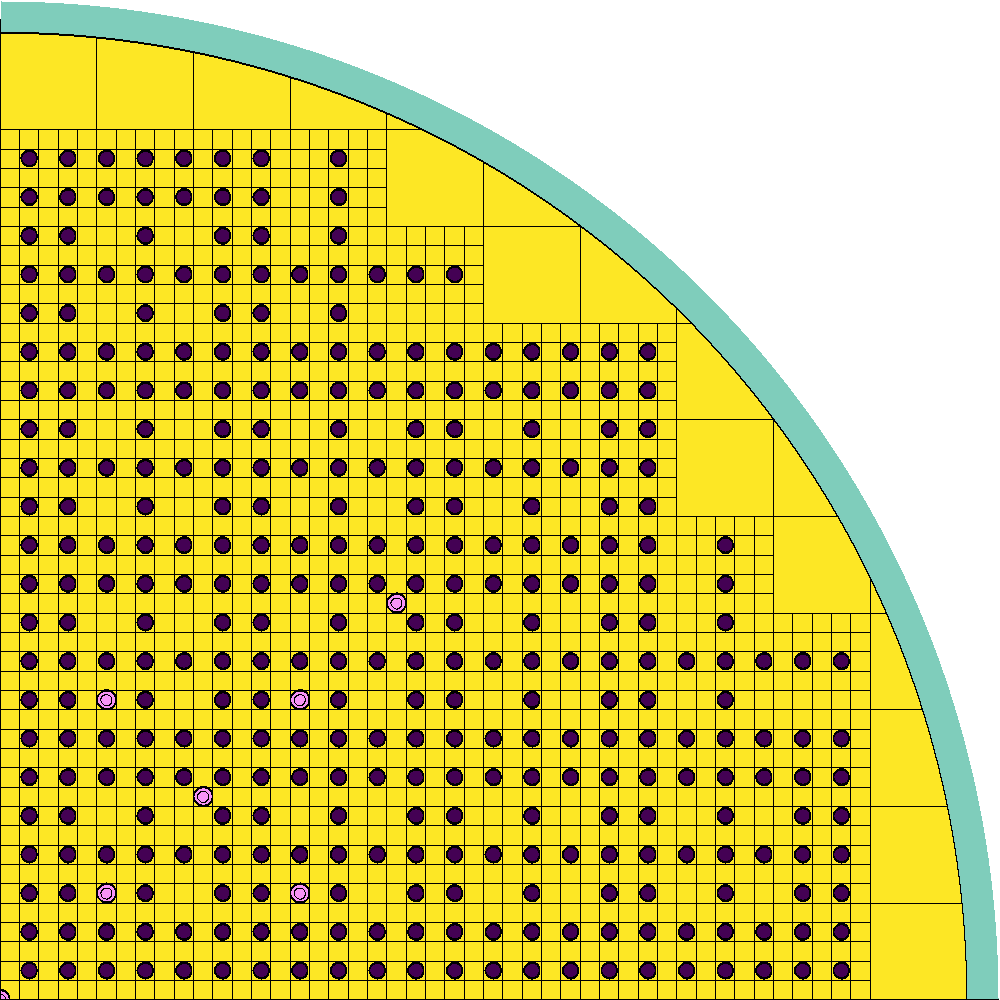
\includegraphics[width=\linewidth]{tap_plan_view.png}
        \caption{The \gls{TAP} \gls{MSR} schematic core view showing moderator 
        rods (figure reproduced from ORNL/TM-2017/475 
        \cite{betzler_assessment_2017}).}
        \label{fig:zoneI}
\end{figure}


%%%%%%%%%%%%%%%%%%%%%%%%%%%%%%%%%%%%%%%%%%%%%%%%%%%%%%%%%%%%%%%%%%%%%%%%%%%%%%%%
\section{Results and Analysis}

Using the methodology described previously, the \gls{MSBR} unit cell depletion 
analysis was performed to find equilibrium core conditions. Calculation results reported 
in this section include multiplication factor, neutron flux energy 
spectrum, and atomic density of major isotopes.

\subsection{Equilibrium state analysis}

This analysis models a single representative unit cell rather than the whole 
\gls{MSBR} core. Consequently, it does not take into consideration different 
fuel-moderator volume ratios for Zone I, Zone II, the annulus, and the reflector. The 
initial multiplication factor during depletion calculation is selected for 
a state with fully withdrawn control rods, which gives 
considerable excess reactivity in the beginning of the cycle (approximately 5000 pcm). 
The standard deviation for these calculations is approximately 100 pcm. Figure~\ref{fig:keff} 
shows the infinite multiplication factor for 1200-days reprocessing cycle calculated by 
Serpent 2 with ENDF/B-VII.0 nuclear data. A significant standard deviation causes the 
multiplication factor fluctuations visible in this plot.

\begin{figure}[htbp!] % replace 't' with 'b' to force it to be on the bottom
	\centering
	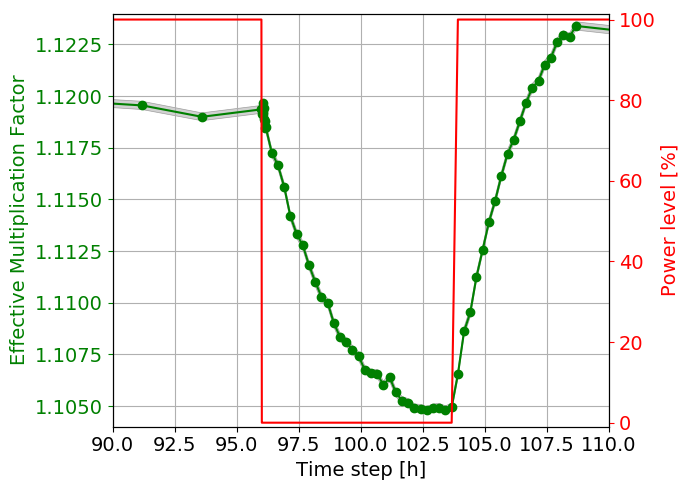
\includegraphics[width=\linewidth]{pwr_keff_zoomed.png}
	\caption{The \gls{TAP} \gls{MSR} schematic core view showing moderator 
		rods (figure reproduced from ORNL/TM-2017/475 
		\cite{betzler_assessment_2017}).}
	\label{fig:zoneI}
\end{figure}
\begin{figure}[htbp!] % replace 't' with 'b' to force it to be on the bottom
	\centering
	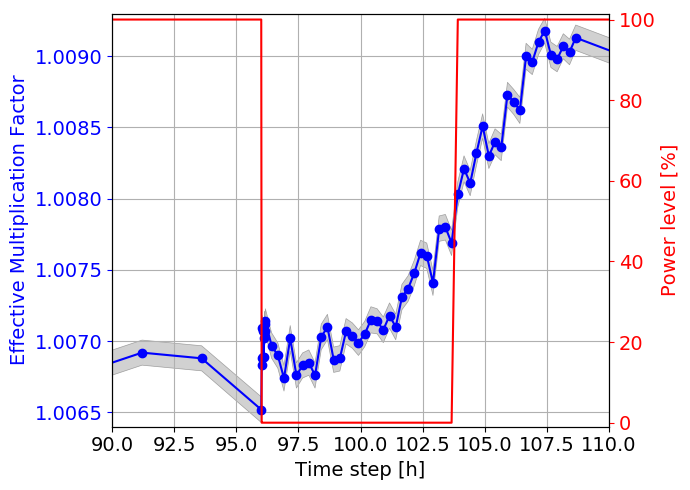
\includegraphics[width=\linewidth]{tap_keff_zoomed.png}
	\caption{The \gls{TAP} \gls{MSR} schematic core view showing moderator 
		rods (figure reproduced from ORNL/TM-2017/475 
		\cite{betzler_assessment_2017}).}
	\label{fig:zoneI}
\end{figure}
\begin{figure}[htbp!] % replace 't' with 'b' to force it to be on the bottom
        \centering
        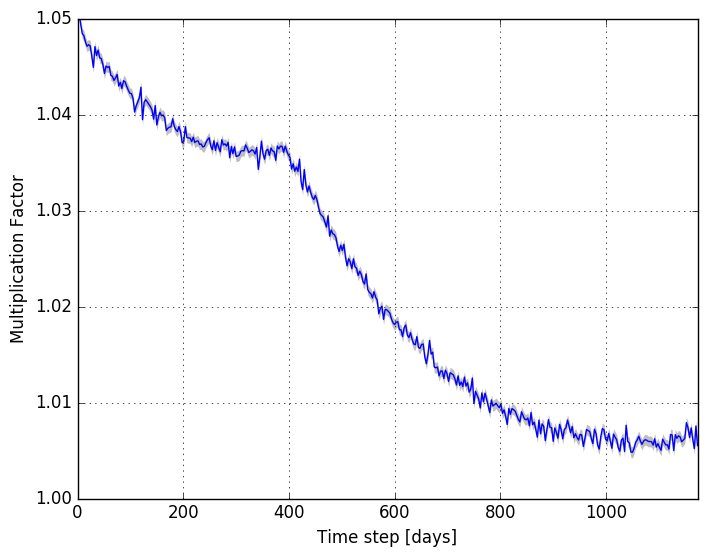
\includegraphics[width=1.05\linewidth]{keff.png}
        \caption{Infinite multiplication factor during a 1200 days depletion
        simulation.The confidence interval $\pm\sigma$ is shaded.}
        \label{fig:keff}
\end{figure}

\FloatBarrier

Protactinium-233 is continuously removing into the tank for protactinium decay.  $^{233}$Pa has a half-life of 27 days and 
beta decays into $^{233}$U which as fresh fuel goes back to the reactor core. 
The infinite multiplication factor decreases first 400 days of depletion due to 
strong absorbers (e.g. $^{233}$Th, $^{234}$U) accumulation which causes 
relatively high fuel ($^{233}$U) refill inflow to keep reactor critical. During 
reactor operation producing fissile materials other than $^{233}$U in the core 
(e.g. $^{235}$U, $^{239}$Pu) which makes it possible to decrease fresh fuel 
refill rate after ~1 year of operation.

\begin{figure}[htbp!] % replace 't' with 'b' to force it to be on the bottom
        \centering
        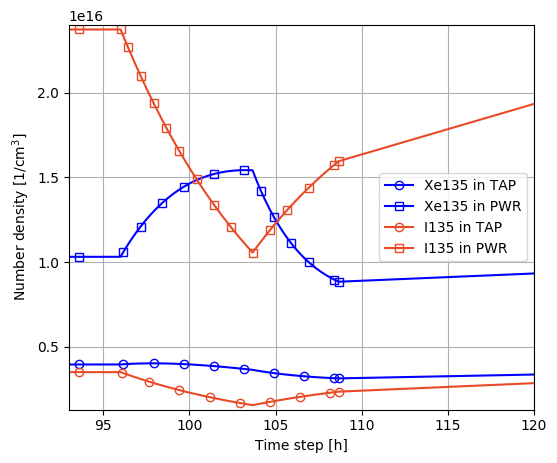
\includegraphics[width=1.05\linewidth]{tap_vs_pwr_xe_i_density.png}
        \caption{Normalized number density of major isotopes during 1200 days of 
        depletion.}
        \label{fig:compos}
\end{figure}

\FloatBarrier

The analysis of the fuel salt composition variation gives clearer information 
about the equilibrium core state. Figure~\ref{fig:compos} shows the normalized 
number density of isotopes influential to core 
neutronics at the beginning of each depletion time interval. The number density 
of protactinium is very low (less than 10$^{16}$ 1/cm$^3$) but some small amount 
of it is produced during the 3-day reprocessing period. In this assessment, the multiplication 
factor stabilizes after approximately 950 days. 
Figure~\ref{fig:rates} represents the rates of online reprocessing material flows
flows over the 4-year depletion calculation. 
In Figure~\ref{fig:rates} we can see that, to keep the reactor critical, a 
higher $^{233}$U 
flow rate from the protactinium decay tank was required for first 400 days of 
operation. After that, the $^{233}$U flow rate can be reduced. The $^{232}$Th 
rate slightly decreases over 4 years of operation due to other than $^{233}$U 
fissile materials accumulation.

As shown in Figure~\ref{fig:outflow}, the tank for protactinium decay 
accumulates $^{233}$Pa for approximately 200 days. Fresh $^{233}$U fuel flow is 
also established after 200 days. Uranium produced in the tank by protactinium 
decay is separated by circulation of the salt through a flourinator. The fully 
processed molten salt, on its way back to the primary loop, has uranium added 
at the rate required to maintain or adjust the fissile material concentration 
and, hence, the reactivity, in the reactor core as desired.

\subsection{Neutron spectrum}

Figure~\ref{fig:spectrum} represents the neutron flux per lethargy energy distribution 
of the initial and the equilibrium core compositions. The spectrum for the 
equilibrium state is harder than the initial state due to heavy fission 
products.  
\begin{figure}[htbp!] % replace 't' with 'b' to force it to be on the bottom
        \centering
        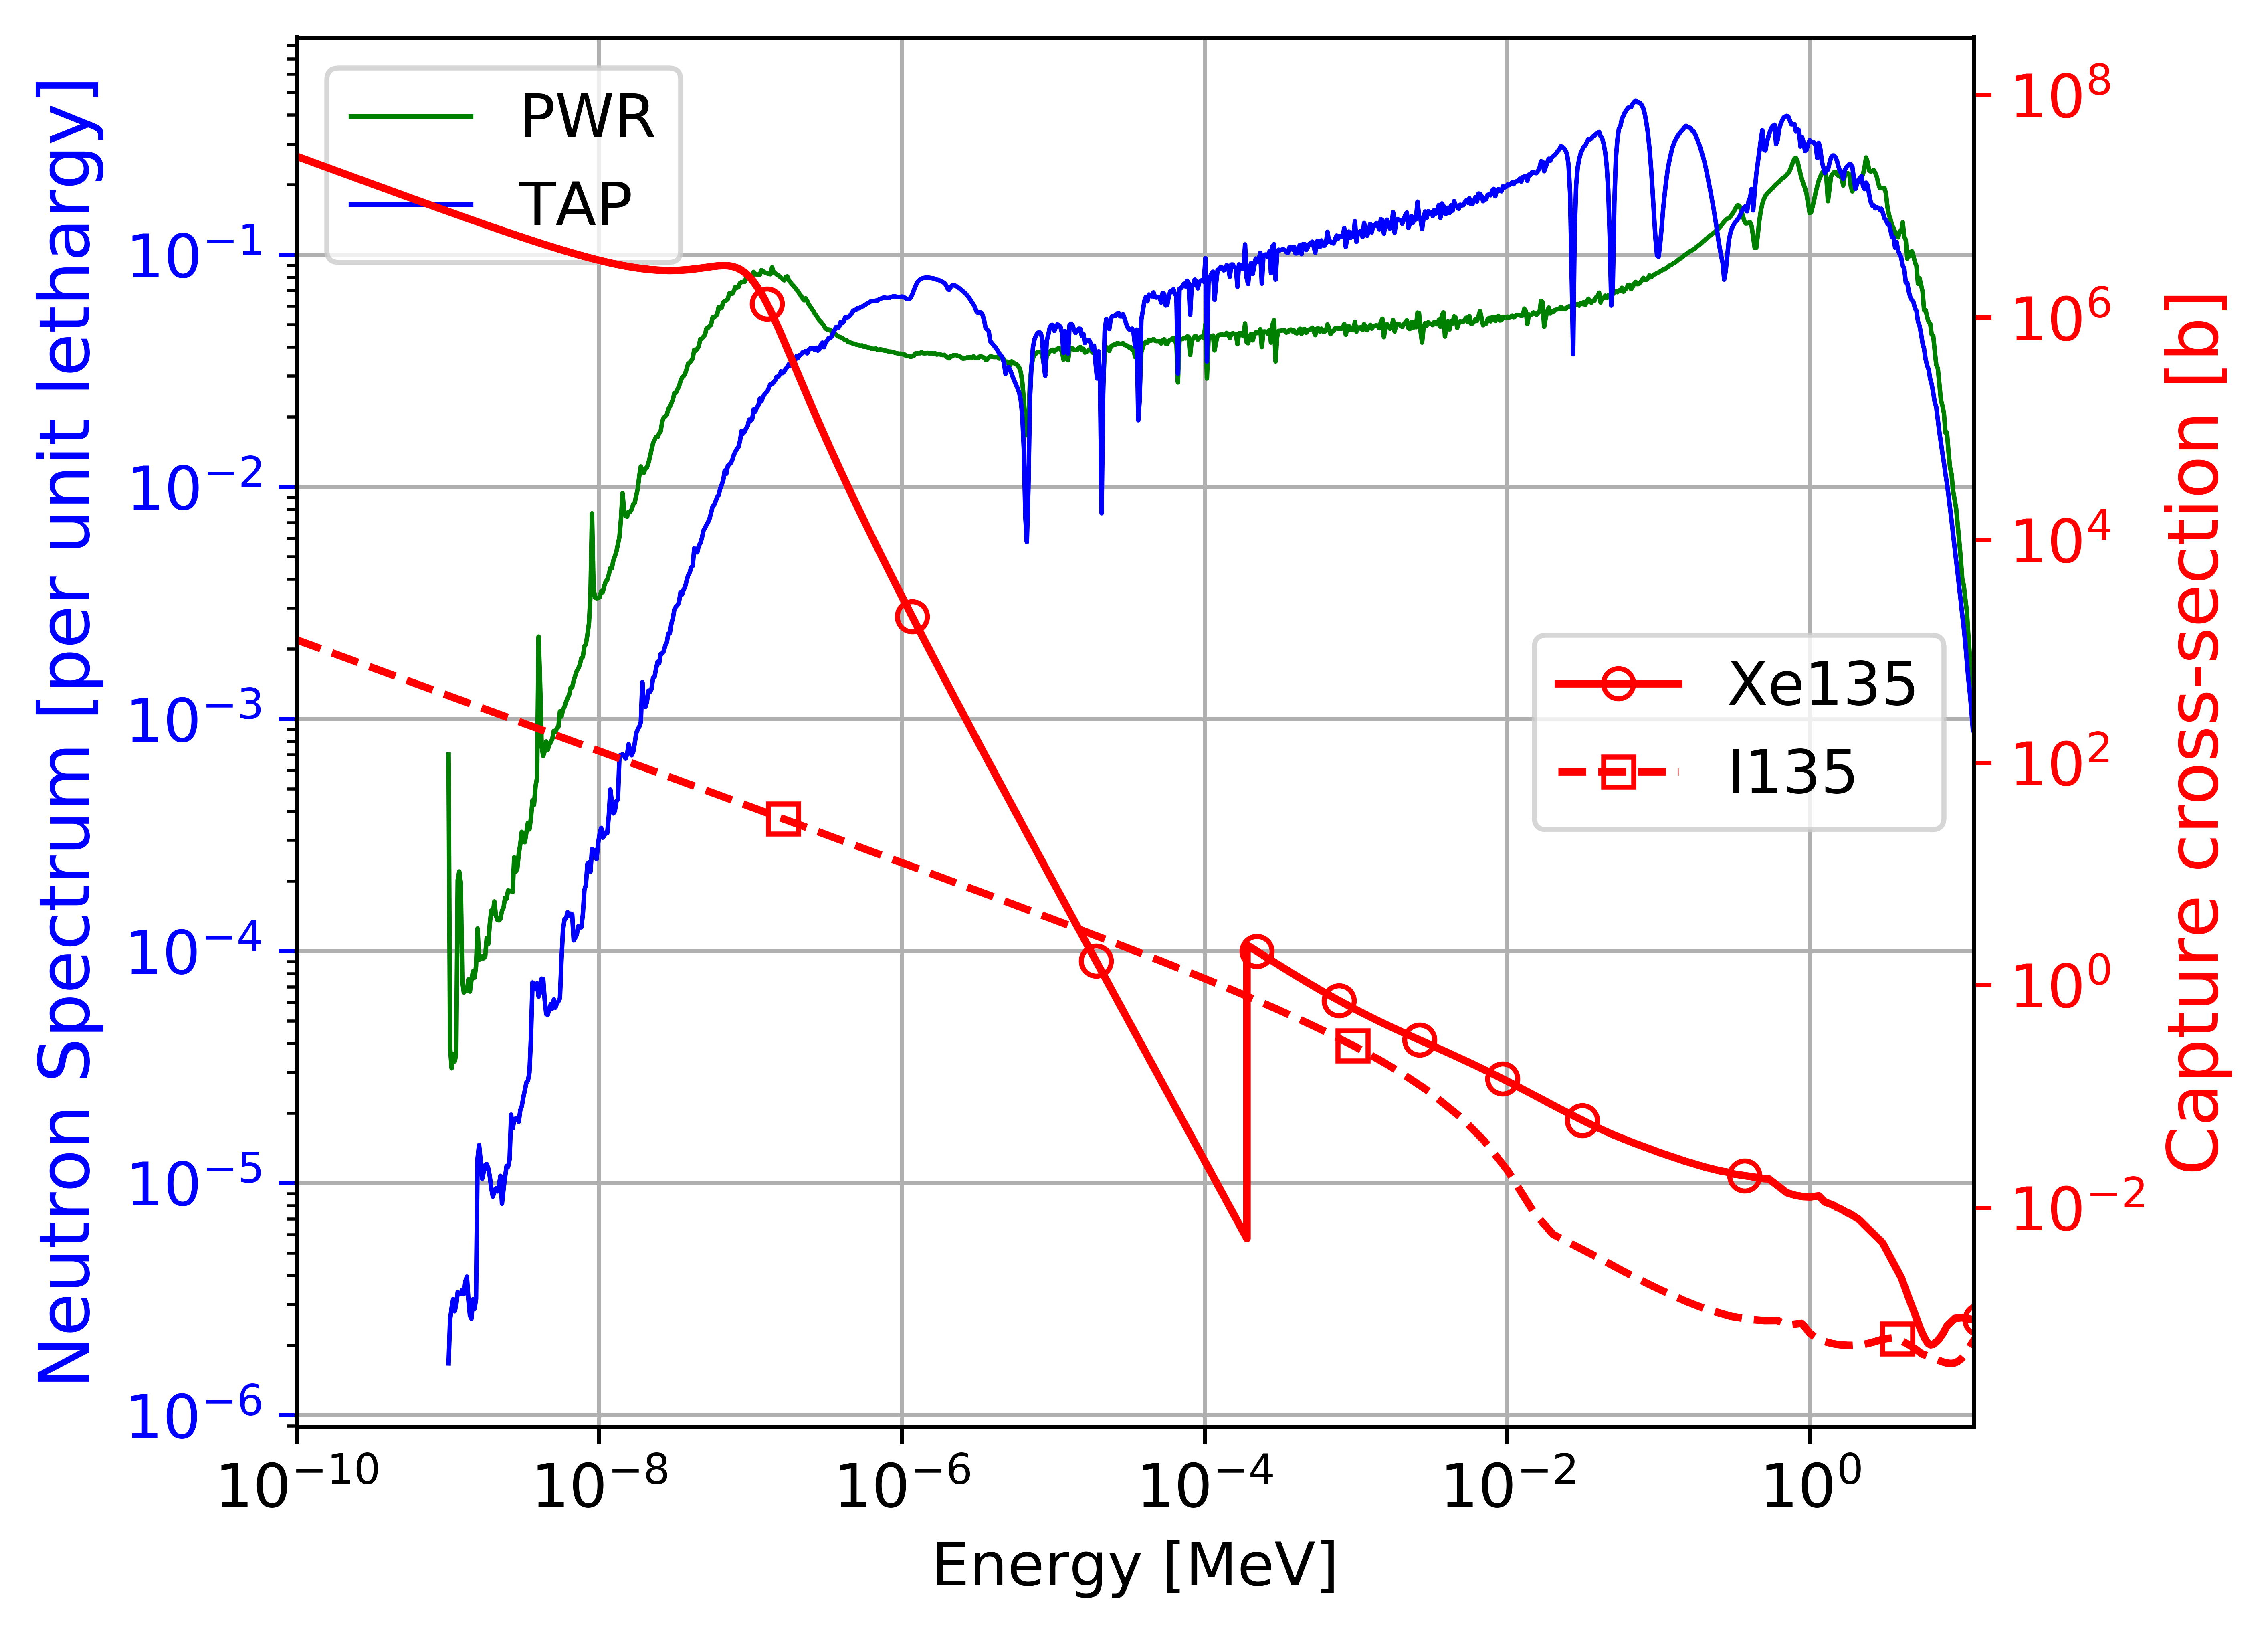
\includegraphics[width=1.05\linewidth]{spectra.png}
        \caption{Neutron spectra for PWR and TAP vs $^{135}$Xe and $^{135}$I 
        caption cross-section.}
        \label{fig:spectrum}
\end{figure}

\FloatBarrier 

In this work, only the Zone I unit cell, where the fuel salt volume fraction is 
13.2\%, was considered. The neutron spectrum for Zone II cell, where the fuel 
salt volume fraction is 37\% is expected to be harder and the peak in thermal 
energy region is predicted to be much 
lower. To obtain a high-fidelity neutron energy spectrum, a full-core \gls{MSBR}
analysis is required.
%%%%%%%%%%%%%%%%%%%%%%%%%%%%%%%%%%%%%%%%%%%%%%%%%%%%%%%%%%%%%%%%%%%%%%%%%%%%%%%%
\section{Conclusions}
The depletion calculation of the \gls{MSBR} unit cell model for finding the 
equilibrium states was performed using the Serpent 2 Monte Carlo code to 
simulate simplified case of the online reprocessing and refueling to find 
equilibrium material composition. When running depletion calculation, the 
fission products are removed and fertile/fissile materials are added to fuel 
salt every 3 days. The important MSR feature, online reprocessing \& refueling 
is implemented in the Serpent 2 material burnup routine. The results of this 
study indicate that from the depletion calculation the multiplication factor 
slowly decreases and reaches to the equilibrium state. The most obvious finding 
to emerge from the analysis of initial and equilibrium materials composition is 
that neutron energy spectrum is harder for equilibrium state because 
significant amount of heavy fission products were accumulated in the \gls{MSBR} 
core.

These results are contrary with those of Jeong and Park (2016) who suggested 
two different unit cell models and uses \gls{MCNP} with Python-script to 
simulate \gls{MSBR} online reprocessing to find equilibrium composition. This 
inconsistency may be due to different fuel fraction in the unit cell (Jeong and 
Park selected 20.6\% salt fraction). To obtain better results for this online 
reprocessing simulation, many future efforts are planned. First, a depletion 
simulation will be performed using a  full-core, three-dimensional, high-fidelity 
model of \gls{MSBR} that has been developed in Serpent 2. In this case, different 
fuel-moderator volume ratios for the reactor Zone I, Zone II, annulus, 
and reflectors will be taken into account to find accurate multiplication factor, 
neutron spectrum and, hence, depleted composition. Secondly, an additional Serpent 
2 flow control system subroutine should be developed to simulate adjusting 
material flows (e.g. rate of removing $^{233}$Pa from the salt and adding 
fissile $^{233}$U from the tank for protactinium decay) depending upon the 
instantaneous reactivity value, which is a more promising reactivity control method than moving 
control rods. Finally, the temperature effect of reactivity for both 
fuel salt and graphite should be calculated to find optimal effective 
multiplication factor range. 

%%%%%%%%%%%%%%%%%%%%%%%%%%%%%%%%%%%%%%%%%%%%%%%%%%%%%%%%%%%%%%%%%%%%%%%%%%%%%%%%
\bibliographystyle{ans}
\bibliography{2019-rykhl-xenon-ans}
\end{document}

